\chapter{Dressed Atom Picture}\label{ch:DressedApproach}

To calculate shifted eigenstates, the full Hamiltonian has to be considered, included a quantized light field with Hamiltonian $\mathcal{H}_L$. This is elegantly treated in \cite{Dalibard1985}.

\begin{equation}
	\mathcal{H} = \mathcal{H}_A + \mathcal{H}_L + \mathcal{H}_I(t)
\end{equation}

where the light field has eigenenergies separated by the photon energy and eigenstates of $n$ photons: $\ket{n}$ \cite{Vredenbregt2020}

\begin{equation}\label{eq:RadiationModes}
	\mathcal{H}_L = \sum_n \hbar \omega \left(n+\frac{1}{2}\right) \ket{n}\bra{n}
\end{equation}

The eigenmodes of the light field can only couple to one energy pair of the $\mathcal{H}_A + \mathcal{H}_I$ part, such that the Hamiltonian can be written down as a direct product of 2 x 2-matrix Hamiltonians \cite{Vredenbregt2020,Hussin2005} $\mathcal{H}_n$:

\begin{equation}\label{eq:CunningsHamiltonian}
    \mathcal{H}_n = \hbar 
    \begin{pmatrix}
        (n + 1)\omega -\omega_0 / 2                     & -\frac{1}{2}\sqrt{\Omega^2+\delta^2(n+1)} \\
        -\frac{1}{2}\sqrt{\Omega^2 + \delta^2(n+1)}  & n\omega + \omega_0/2
    \end{pmatrix}
\end{equation}

This is known as the Jaynes-Cummings Hamiltonian, which is one of the few problems in quantum optics analytically solvable.
It has eigenvalues \cite{Hussin2005}

\begin{equation}\label{eq:CunningsEigenvalues}
    E_{\pm} = \hbar\omega\left(n+\frac{1}{2}\right) \pm \frac{\hbar}{2} \sqrt{\delta^2 + \Omega^2(n+1)}.
\end{equation}

From \cref{eq:CunningsEigenvalues} the new eigenstates can be found to be \cite{Hussin2005}

\begin{subequations}\label{eq:CummingsEigenstates}
    \begin{align}
        \ket{+,n} &= \cos{({\theta_n}/2)} \ket{n+1,g} -\sin{(\theta_n/2)} \ket{n,e}, \\
        \ket{-,n} &= \sin{(\theta_n/2)}\ket{n+1,g} + \cos{(\theta_n/2)} \ket{n,e}.
    \end{align}
\end{subequations}

Which are sketched in \cref{fig:DressedStatePicture} as well. 
In \cref{eq:CummingsEigenstates} the mixing angle $\theta_n$ for $n$ photons in the system is $\theta_n = \arctan{(\Omega\sqrt{n+1} / \delta})$.
Here, \cref{eq:CummingsEigenstates} are known as the \emph{dressed} states.
The \emph{bare} atomic states in \cref{fig:2LevelAtom} are shifted by the light shift because the light field energy is admixed with the atomic eigenstates, leading to the new mixed (dressed) eigenstates of \cref{eq:CummingsEigenstates}. 
The bevavior pictured in \cref{fig:DipoleForce} still applies, but if the eigenenergies of the light field are included, the splitted energies of \cref{fig:DipoleForce} are situated along an infinite ladder of photon energies. 
This is presented in \cref{fig:DressedStatePicture}. 
The light space eigenenergies \cref{eq:RadiationModes}, spaced by $\hbar \omega$ is superimposed on the light shift eigenenergies. 

\begin{figure}
    \centering
    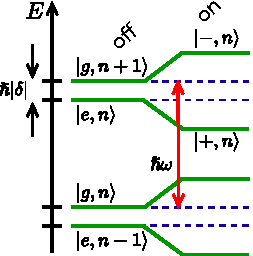
\includegraphics[width=0.4\linewidth]{figures/DressedStates.pdf}
    \caption{Dressed States. The same shift as shown in \cref{fig:DipoleForce} is shown, superimposed on the  eigenenergies spaced by $\hbar \omega$. 
    Figure not to scale. }
    \label{fig:DressedStatePicture}
\end{figure}
